\clearpage\begingroup\SourceLeaf{382b}\ArithmeticHead{51}{R}{GEOMETRIA SITUS.}
\renewcommand{\thefootnote}{\arabic{footnote})}\setcounter{footnote}{1}
\begin{center}
\textbf{13.}\par\smallskip
\textsc{Möbius, Listing, Riemann.}
\end{center}
\noindent\hspace*{\parindent}Mit der Frage, welchen Einfluss \textsc{Gauss} auf die weitere Entwicklung der
Geometria situs gehabt hat, kommen wir auf ein schwieriges Gebiet, denn
ein solcher Einfluss war im Wesentlichen nur möglich durch mündliche
Äusserungen, von denen manche, wie es scheint, gar erst durch Mittelsleute
an die Stelle gekommen sind, wo sie gewirkt haben; es waren Funken, die
nur da zündeten, wo schlummernde Energien zu wecken waren, und es heisst
daher nicht, hervorragende Männer wie \textsc{Möbius, Listing, Riemann} verkleinern,
wenn man glaubt, \textsc{Gauss} einen gewissen Einfluss auf ihre Entdeckungen zuschreiben
zu müssen.
\par\medskip
\textsc{Möbius} (1790—1868) ist nach Abschluss seiner Leipziger Studien im
Herbst 1813 als Dreiundzwanzigjähriger nach Göttingen gekommen und hat
dort etwa ein Semester lang unter Leitung von \textsc{Gauss} auf der Sternwarte gearbeitet
(Brief von \textsc{Gauss} an \textsc{Olbers} vom 23. April 1814, Br. G.-O. 1, S. 543).
Es war die Zeit, wo man in der Astronomie von einer \textsc{Gauss}schen Schule
sprechen konnte, aus der \textsc{Encke, Gerling, Nicolai, Schumacher, Seeber, Struve,
Wachter} hervorgegangen sind. Dass der junge Sachse damals in nähere Beziehungen
zu \textsc{Gauss} gekommen ist, zeigt der freundschaftliche Ton der Briefe,
\par\nobreak\hfill{\small 7\textsuperscript{*}}
\clearpage\SourceLeaf{383}\ArithmeticHead{52}{L}{STÄCKEL, GAUSS ALS GEOMETER.}\setcounter{footnote}{0}
\noindent die lange Jahre hindurch zwischen ihnen gewechselt worden sind. Es bestand
zwischen \textsc{Gauss} und \textsc{Möbius}, als dieser in Göttingen weilte, jenes Verhältnis,
das \textsc{Gauss} am förderlichsten schien. »Meiner Einsicht nach ist [ein förmlicher
Unterricht] bei solchen Köpfen, die nicht etwa nur eine Masse von Kenntnissen
einsammeln wollen, sondern denen es hauptsächlich daran liegt, ihre
eigenen Kräfte zu üben, sehr unzweckmässig; einen solchen muss man nicht
bei der Hand fassen und zum Ziele führen, sondern nur von Zeit zu Zeit
ihm Winke geben, um sich selbst auf dem kürzesten Wege hinzufinden« (Brief
an \textsc{Schumacher} vom 2. Oktober 1808, Br. G.-Sch. I, S. 6). Wie weit die zahlreichen
Berührungspunkte zwischen den Untersuchungen von \textsc{Möbius} und den
Gedanken von \textsc{Gauss} auf Gespräche oder auch, wie \textsc{Listing} einmal sagt, auf
»hingeworfene Äusserungen« zurückzuführen sind, vielleicht zum Teil in unbewusster
Nachwirkung, entzieht sich unserer Kenntnis. In einem Falle freilich
hat sich \textsc{Möbius} ausdrücklich auf eine mündliche Mitteilung von \textsc{Gauss} bezogen,
nämlich in Aufzeichnungen aus den Jahren 1858 und 1859 über die
Topologie der krummen Flächen und im Besonderen der Polyeder, Aufzeichnungen,
die erst 1886 durch \textsc{Reinhardt} aus dem Nachlass herausgegeben
worden sind\footnote{A. F. \textsc{Möbius}, Gesammelte Werke II, Leipzig 1886, S. 518—559. Einen Teil der darin enthaltenen Ergebnisse hat \textsc{Möbius} veröffentlicht: \textit{Theorie der elementaren Verwandtschaft}, Leipziger Berichte 1863, S. 18, Werke II, S. 433; \textit{Über die Bestimmung des Inhalts eines Polyeders}, ebenda 1865, S. 31, Werke II, S. 473.}. In dem Abschnitt über Flächen und Polyeder höherer Klasse
[mehrfachen Zusammenhanges] werden auch die Eigenschaften eines Doppelringes
betrachtet, und es heisst: »Man kann sich einen solchen Doppelring
leicht zur Anschauung bringen, wenn man ein Blatt Papier in Form eines
\par\nobreak\noindent
\begin{minipage}[t]{.33\linewidth}
\vspace{0pt}\centering
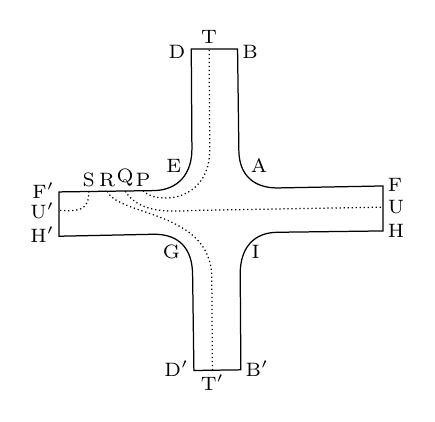
\begin{tikzpicture}[x=.84cm,y=.84cm,line width=.45pt,
every node/.style={font=\scriptsize,inner sep=1pt}]
\draw (-.35,2.4)--(.35,2.4)--(.37,.85)
 .. controls (.38,.48) and (.61,.30) .. (.95,.30)
 --(2.55,.33)--(2.55,-.35)--(.96,-.37)
 .. controls (.59,-.37) and (.40,-.61) .. (.39,-.97)
 --(.40,-2.45)--(-.31,-2.46)--(-.33,-.99)
 .. controls (-.34,-.61) and (-.54,-.40) .. (-.91,-.40)
 --(-2.35,-.43)--(-2.35,.24)--(-.91,.26)
 .. controls (-.55,.27) and (-.34,.51) .. (-.34,.89)--cycle;
\draw[densely dotted] (-1.08,.26)
 .. controls (-.89,.05) and (-.08,.07) .. (-.07,.87)
 --(-.08,2.4);
\draw[densely dotted] (-1.62,.25)
 .. controls (-1.45,-.13) and (-.05,-.04) .. (-.04,-1.05)
 --(-.03,-2.45);
\draw[densely dotted] (-1.35,.25)
 .. controls (-1.13,-.08) and (-.72,-.06) .. (-.30,-.04)
 --(2.55,.01);
\draw[densely dotted] (-1.90,.25)
 .. controls (-1.89,-.06) and (-2.08,-.05) .. (-2.35,-.04);
\node[anchor=east] at(-.39,2.35){D};
\node[anchor=south] at(-.08,2.43){T};
\node[anchor=west] at(.37,2.35){B};
\node[anchor=south east] at(-.45,.48){E};
\node[anchor=south west] at(.50,.48){A};
\node[anchor=east] at(-2.37,.26){F\('\)};
\node[anchor=east] at(-2.37,-.04){U\('\)};
\node[anchor=east] at(-2.37,-.41){H\('\)};
\node[anchor=south] at(-1.90,.27){S};
\node[anchor=south] at(-1.62,.27){R};
\node[anchor=south] at(-1.35,.27){Q};
\node[anchor=south] at(-1.08,.27){P};
\node[anchor=west] at(2.57,.34){F};
\node[anchor=west] at(2.57,.01){U};
\node[anchor=west] at(2.57,-.35){H};
\node[anchor=north east] at(-.47,-.52){G};
\node[anchor=north west] at(.51,-.52){I};
\node[anchor=east] at(-.34,-2.43){D\('\)};
\node[anchor=north] at(-.03,-2.47){T\('\)};
\node[anchor=west] at(.42,-2.43){B\('\)};
\end{tikzpicture}
\end{minipage}\hfill
\begin{minipage}[t]{.65\linewidth}
\vspace{0pt}\setlength{\parindent}{1.2em}\noindent
Kreuzes ausschneidet und hierauf die Enden \(FH\)
und \(F'H'\) (siehe die Figur) des einen Paares einander
gegenüberliegender Arme etwa oberhalb der
anfänglichen Ebene des Kreuzes und die Enden
\(BD\) und \(B'D'\) des anderen Paares unterhalb dieser
Ebene mit einander vereinigt. Es besitzt diese
nur von einer Linie \(A\overline{BB'}I\overline{HH'}G\overline{D'D}E\overline{F'F}A\)
begrenzte Fläche noch die merkwürdige Eigenschaft
(nach einer mündlichen Mitteilung von \textsc{Gauss};
\end{minipage}
\clearpage\SourceLeaf{384}\ArithmeticHead{53}{R}{GEOMETRIA SITUS.}\setcounter{footnote}{0}
\noindent wodurch G. zur Betrachtung der Fläche geführt worden ist, ist mir unbekannt),
dass man von irgend vier auf ihrem Perimeter auf einander folgenden
Punkten \(P, Q, R, S\) den ersten mit dem dritten und den zweiten mit dem
vierten durch zwei Linien \(P\overline{TT'}R\) und \(Q\overline{UU'}S\) verbinden kann, welche in
der Fläche selbst liegen und dennoch einander nicht schneiden, — wie dies
doch immer geschehen würde, wenn die Fläche eine Grundform der ersten
Klasse [einfach zusammenhängend] wäre« (S. 541).
\par
Als die Fürstlich \textsc{Jablonowski}sche Gesellschaft der Wissenschaften zu
Leipzig im Jahre 1844 die Preisaufgabe gestellt und, nachdem keine Lösung
eingelaufen war, 1845 wiederholt hatte: »Es soll nach den vorhandenen Bruchstücken
die von \textsc{Leibniz} geplante geometrische Charakteristik wiederhergestellt
und weiter ausgebildet werden«, hat \textsc{Möbius Grassmann} darauf hingewiesen,
und dessen Abhandlung: \textit{Geometrische Analyse} hat am 1. Juli 1846 auf den
eingehend begründeten Antrag von \textsc{Drobisch} und \textsc{Möbius} den Preis erhalten\footnote{Vgl. \textit{Grassmanns Leben} von F. \textsc{Engel}, \textsc{Grassmanns} Werke III, Teil 2, Leipzig 1911, S. 108—118. Die Abhandlung ist abgedruckt in den Werken Bd. I, Teil 1, S. 321—399.}.
\textsc{Möbius} hat am 2. Februar 1847 einen Abdruck der Preisarbeit an \textsc{Gauss} gesandt\footnote{\textsc{Grassmanns} Werke III, Teil 2, S. 117.},
sicherlich in der Annahme, dass dieser an dem Gegenstande Anteil
nehme.
\par
Weiteres über Beziehungen zwischen Gedanken von \textsc{Gauss} und von \textsc{Möbius}
findet man im vierten Abschnitt dieses Aufsatzes.
\par\medskip
\textsc{Listing} (1806—1882) hatte in Göttingen Mathematik und Naturwissenschaften
studiert und war dort 1834 unter dem Dekanat von \textsc{Gauss} mit einer
Abhandlung über die Flächen zweiter Ordnung promoviert worden. Noch in
demselben Jahre schloss er sich \textsc{Sartorius} v. \textsc{Waltershausen} auf einer Reise
nach Sizilien an und wurde sein Gehilfe bei den geologischen Untersuchungen
am Aetna. Nach Deutschland zurückgekehrt ist er seit 1837 als Lehrer der
Maschinenkunde am Polytechnikum zu Hannover und seit 1839 als Professor
der Physik an der Universität Göttingen tätig gewesen.
\par
Der Nachlass \textsc{Listings}\footnote{Die betreffenden Aufzeichnungen besitzt teils die Universitätsbibliothek in Göttingen, teils der Verfasser dieses Aufsatzes.} zeigt, dass er sich schon früh mit dem »Knotenwesen«
und seinen Beziehungen zur Praxis der Seeleute und der Pioniere
\clearpage\SourceLeaf{385}\ArithmeticHead{54}{L}{STÄCKEL, GAUSS ALS GEOMETER.}\setcounter{footnote}{0}
\noindent befasst hat. In einem Briefe an einen gewissen \textsc{Müller} in Göttingen, datiert
Catania, den 1. April 1836, schreibt er: »Die erste Idee, mich in der Sache
[der Geometria situs] zu versuchen, ist mir durch allerlei Vorkommnisse bei
den praktischen Arbeiten auf der Sternwarte in Göttingen und durch hingeworfene
Äusserungen von \textsc{Gauss} beigekommen«. Dass \textsc{Gauss} in den Vorlesungen
über praktische Astronomie die Geometria situs berührt hat, bezeugt
die \textit{Theorie des Vortrags von Lehren, die Raumverhältnisse betreffen}, W. VIII,
S. 196—199.
\par
In demselben Sinne schreibt \textsc{Listing} in einer 1856 verfassten kurzen
Lebensbeschreibung: »Einen andern Gegenstand meiner Beschäftigung bildet
seit langer Zeit die Untersuchung der modalen (nichtquantitativen) Raumverhältnisse,
zu der schon \textsc{Leibniz} die Idee gefasst hatte. Ich habe zu dieser
fast noch ganz unausgebauten quasi-mathematischen Disziplin, zum Teil durch
\textsc{Gauss} aufgemuntert, in den \textit{Vorstudien zur Topologie}, Göttingen 1847, einen
ersten Versuch veröffentlicht, dem ich künftig noch andere hoffe folgen lassen
zu können«.
\par
Nach seinen Aufzeichnungen hat \textsc{Listing} schon während des Aufenthalts
in Italien, seit 1835, begonnen, sich mit der \textls[100]{Topologie} zu beschäftigen; so
wollte er die Lehre von den »qualitativen Gesetzen der örtlichen Verhältnisse«
genannt wissen, weil der Name Geometrie der Lage schon in anderer Bedeutung
verwendet werde. Der lange Brief an \textsc{Müller} vom 1. April 1836
beweist, dass er bereits damals im Wesentlichen zu den Ergebnissen gelangt
war, die er 1847 in der Zeitschrift »Göttinger Studien« als Abhandlung und
dann 1848 als besondere Schrift veröffentlicht hat. Dass er im Jahre 1845
seine Beschäftigung mit der Topologie wieder aufnahm und nunmehr zu einem
ersten Abschluss kam, ist wohl auf eine Anregung von \textsc{Gauss} zurückzuführen,
denn in den tagebuchartigen Notizen, den »Diarien«, die \textsc{Listing} geführt hat,
ist unter dem 2. Januar 1845 verzeichnet; »Bei \textsc{Gauss}, Geometria situs«.
\par
Mit dem Jahre 1858 beginnt eine neue Reihe topologischer Untersuchungen,
die zu der grossen, 1862 erschienenen Abhandlung über den \textit{Census räumlicher
Complexe} geführt haben. Das Ziel \textsc{Listings} war, dem \textsc{Euler}schen Satze über
die Beziehung zwischen den Anzahlen der Ecken, Kanten und Flächen eines
Vielfachs, der nur unter einschränkenden Voraussetzungen richtig ist, eine
allgemein gültige Form zu geben. Merkwürdigerweise hat in demselben
\clearpage\SourceLeaf{386}\ArithmeticHead{55}{R}{GEOMETRIA SITUS.}\setcounter{footnote}{0}
\noindent Jahre 1858 auch \textsc{Möbius} begonnen, sich mit der Geometria situs der Polyeder
zu beschäftigen\footnote{Vgl. die Bemerkung \textsc{Reinhardts}, \textsc{Möbius} Werke II, S. 519.}, und beide, \textsc{Listing} und \textsc{Möbius}, sind fast gleichzeitig und
unabhängig von einander zur Entdeckung der einseitigen Flächen gelangt\footnote{Vgl. P. \textsc{Stäckel}, \textit{Die Entdeckung der einseitigen Flächen}, Math. Annalen, Bd. 52, 1899, S. 598.}.
\par
Den Schlüssel zur Verallgemeinerung des \textsc{Euler}schen Satzes bildet der
Begriff des \textls[100]{Zusammenhangs} oder, wie \textsc{Listing} mit einem nicht üblich gewordenen
Worte sagt, der Cyklose, die einem irgendwie berandeten Flächenstücke
zukommt. Dass \textsc{Gauss} den Begriff des Zusammenhanges und seine
Bedeutung für die Lehre von den Funktionen einer komplexen Veränderlichen
erkannt hat, zeigt das aus dem Nachlass herausgegebene Bruchstück über die
Konvergenz der Entwicklungen periodischer Funktionen (W. X\textsubscript{1}, S. 410—412),
das um das Jahr 1850 entstanden ist. Auch die bereits erwähnte mündliche
Mitteilung an \textsc{Möbius} über den Doppelring und die darauf liegenden Kurven
gehört hierher. Ob \textsc{Listing} durch Äusserungen von \textsc{Gauss} auch zur Fortsetzung
seiner Untersuchungen über die Topologie angeregt worden ist, muss
dahingestellt bleiben. Ebenso ist das Verhältnis, in dem die Arbeiten von
\textsc{Riemann} über die Analysis situs\footnote{B. \textsc{Riemann}, \textit{Grundlagen für eine allgemeine Theorie der Functionen einer veränderlichen complexen Grösse}, Dissertation, Göttingen 1851, art. 6; Werke, 1. Aufl., S. 9—12; \textit{Theorie der Abelschen Functionen}, zweiter Abschnitt, \textsc{Crelles} Journal, Bd. 54, 1857, Werke, 1. Aufl., S. 84—89.} zu den topologischen Untersuchungen von
\textsc{Listing} stehen, noch ungeklärt.
\par
Während bei \textsc{Möbius} und \textsc{Listing} eigene Zeugnisse vorliegen, dass sie
durch \textsc{Gauss} zur Beschäftigung mit der Geometria situs angeregt worden seien,
obwohl nicht festgestellt werden kann, in welchem Umfange das geschehen
sein mag, sind wir bei \textsc{Riemann} (1826—1866) lediglich auf Vermutungen angewiesen.
Ein unmittelbarer Verkehr mit \textsc{Gauss} kommt kaum in Betracht,
wohl aber darf man an eine Vermittlung \textsc{Gauss}scher Gedanken durch A. \textsc{Ritter}
(1826—1908) und W. \textsc{Weber} (1804—1891) denken. \textsc{Ritter} hat während
seiner Göttinger Studienzeit, 1850 bis 1853, in engen Beziehungen zu \textsc{Riemann}
gestanden, die sich später fortsetzten; es ist anzunehmen, dass \textsc{Riemann}
durch ihn Kenntnis erhalten hat zum Beispiel von den Ausführungen, die
\textsc{Gauss} in der Vorlesung über die Methode der kleinsten Quadrate im Wintersemester
1850/51 über \(n\)-dimensionale Mannigfaltigkeiten gemacht hat (W. X\textsubscript{1},
\clearpage\SourceLeaf{387a}\ArithmeticHead{56}{L}{STÄCKEL, GAUSS ALS GEOMETER.}\setcounter{footnote}{0}
\noindent S. 473—482). Mit \textsc{Weber} aber stand \textsc{Riemann} seit 1850 als Teilnehmer, seit
1853 als Assistent an dessen mathematisch-physikalischem Seminar in engem
Verkehr\footnote{Vgl. die Bemerkungen \textsc{Dedekinds} in \textsc{Riemanns} Lebenslauf, Werke, 1. Aufl., S. 512—515.}, und wir haben aus dem Briefe von \textsc{Möbius} an \textsc{Gauss} vom 2. Februar
1847 erfahren, dass dieser mit \textsc{Weber} über die Umschlingungen zweier
Kurven im Raume gesprochen hatte. Wie dem aber auch sei, so gibt es
kein Anzeichen, dass \textsc{Gauss} den Begriff der mehrblättrigen Fläche, die zur
Darstellung des Verlaufs einer mehrdeutigen Funktion einer komplexen Veränderlichen
dient, gekannt habe, und hier liegt also sicher eine durchaus ursprüngliche
Schöpfung \textsc{Riemanns} vor.
\par\medskip\centerline{\rule{.2\linewidth}{.35pt}}
\clearpage\endgroup

